\chapter{Method}


Several hypotheses were tested in this work.
Section \ref{data} gives an overview of how input data was pre-processd.
Section \ref{architecture} describes the technical set up required for running all these experiments and deploying the model to production before delving into the specific experiments and their evaluation methods in sections [ref].

\hfill \break \noindent
The experiments were conducted in four distinct stages:

 \begin{itemize}
   \item Training a baseline model on the rule-based labels to get a sense of the difficulty of this problem. Since there is no fundamental difference in the way this model was  trained and evaluated compared to the other classifiers, this is described in section \ref{exp_models} with the others. After this step, employees of the client company labeled products that would become the ground truth dataset. The visual comparison feature was also subjectively evaluated at this stage.
   \item Training the independent classifiers to determine best performers (\ref{exp_models}).
   \item Training an ensemble of the independent classifiers (\ref{exp_ensembling}).
   \item Training up to 10 iterations of active learning on the strong predictor (\ref{exp_al}).
 \end{itemize}


 \section{Data Preprocessing}
 \label{data}

There were around a dozen product features that affiliate network provided.
Most of these features were either categorical or textual,  with just a single numerical feature (price).
The initial analysis of the dataset was performed using Dataprep, a Google Cloud Platform (GCP)  product for data wrangling, which at the time of use was in beta stage.
Dataprep  was used to process a sample of ~800 000 products;  it produced histograms of the values present in each feature column (see appendix \ref{dataprep}), which was used  to determine which input features to discards entirely.


 config file for how to preprocess data
 selecting top\_k for each column
 input representation: 1-hot, k-hot, tfidf, embedding

 \subsection{Category Structure}
 \label{cat_tree}


\section{System Architecture}
\label{architecture}

 The following technologies were used to build the system which had to interact with existing services  at the client company:

\begin{itemize}
  \item Apache Airflow (AF) - a Python framework for defining workflows of long-running tasks and dependencies between these tasks.
  \item TensorFlow (TF) - ML framework for Python, capable of defining many kinds of models as a computation graph, and executing this graph locally or in a distributed manner.
  \item ML Engine (MLE) - a GCP service for running TensorFlow models (training, hyperparameter tuning, inference).
  \item Apache Beam - a data processing engine akin akin to Apache Spark and Apache Flink.
  \item Dataflow - a GCP service for executing Apache Beam workloads.
  \item Tensorflow Transform - a Python library with a small set of operations for data preprocessing that can run inside a TensorFlow graph as well as an Apache Beam pipeline.
  \item Google Cloud Storage (GCS) - Google Cloud Platform (GCP) object storage similar to Amazon S3.
  \item ElasticSearch (ES) - a NoSQL database with powerful full-text search and querying capabilities.
  \item RabbitMQ - a message queue, used for transferring data among our microservices (using the Logstash adapter, that can read from and write to (among other things) ElasticSearch and RabbitMQ).
  \item Flask - a simple backend web framework for Python.
  \item Node.js - a JacaScript backend web framework.
  \item React.js - a JavaScript front-end framework for JavaScript.
  \item Redux - a framework for persisting user interface (UI) state and application data in single page applications.
  \item GraphQL - a query language for building flexible APIs
\end{itemize}

Figure \ref{arch_diagram} shows the how data is passed between the main services, and how services and technologies interact.

All product data is stored in ElasticSearch (ES): the rule-based labels, the predictions of the ML system, and evaluation metrics from various train runs.
ES is accessed from the public web application via GraphQL and the ML administration web UI (further referred to just as web UI).
The web UI was initially built with Flask and React by the author as a quick way to get insight about the model, and then re-written as a more feature-rich version by an employee of the client company with Node.js, GraphQL, React and Redux.
Data is pulled into the ML pipelines by dumping the results of an ES query to a local file, which is uploaded to GCS.
Updates to the ES index are not done directly, since indexing the updated products is computationally expensive; instead, updates are put on a RabbitMQ queue, which is consumed by Logstash, which updates products in ES at a rate that will not overburden the servers.

All ML training and prediction happens in a batch-oriented way, encapsulated as Airflow pipelines.
Each pipeline is a directed acyclic graph of tasks, where a task can be a shell command or Python function; a pipeline defines dependencies of task execution, which allows us co-ordinate a series of operations that could be executed locally inside the Docker container running AF, or remotely such as in a GCP service.
A typical pipeline dumps data locally, uploads it to GCS, schedules a Dataflow job to preprocess data, polls the Dataflow service until the Dataflow job is finished, schedules an ML engine job, polls the MLE service until it has completed, and runs an update process that reads the predictions and evaluation statistics from GCS and sends the updates to the RabbitMQ queue.
Reading updates and sending these to RabbitMQ is done in a parallelised manner (using multiprocessing), since the update process is bottlenecked due to network latency as well as computing the appropriate category tree for each product (explained in \ref{cat_tree}).

There are two types of Dataflow pipelines: preprocessing and similarity pipelines. Omitting various details, dead-ends and workarounds that were needed due to prior system architecture changes\footnote{which were completely reasonable at the time, when the ML system was not a consideration}, the pipelines had the following tasks:

\begin{itemize}
  \item \textbf{Preprocess pipeline.}
    It loads the products dumped from ES (as JSON) and preprocesses data according to a configuration file (see section \ref{data}).
    All fields are cleaned of obvious noise and superfluous whitespace.
    Numerical fields are normalised, histograms are computed for categorical variables.
    Text fields are tokenised, tokens are counted and used for computing TF-IDF values.
    This tokenisation is handled by TensorFlow Transform: it keeps the top \textit{k} tokens (or categorical values) for a categorical (or text) column, and maps these to integer indices.
    Which tokens (or categorical values) map to which indices determines the 1-hot input encoding of the data (or similar, see section \ref{data}), and will be different every time data is pre-processed again.
    This token-to-index mapping is encoded in a \textit{transform function} that is saved to GCS at the end of the pipeline, and is used by a TensorFlow model to convert raw text inputs to a  sparse inputs.
  \item \textbf{Visual similarity pipeline} -
\end{itemize}

\begin{figure}
  \hspace*{-0.2\textwidth}
  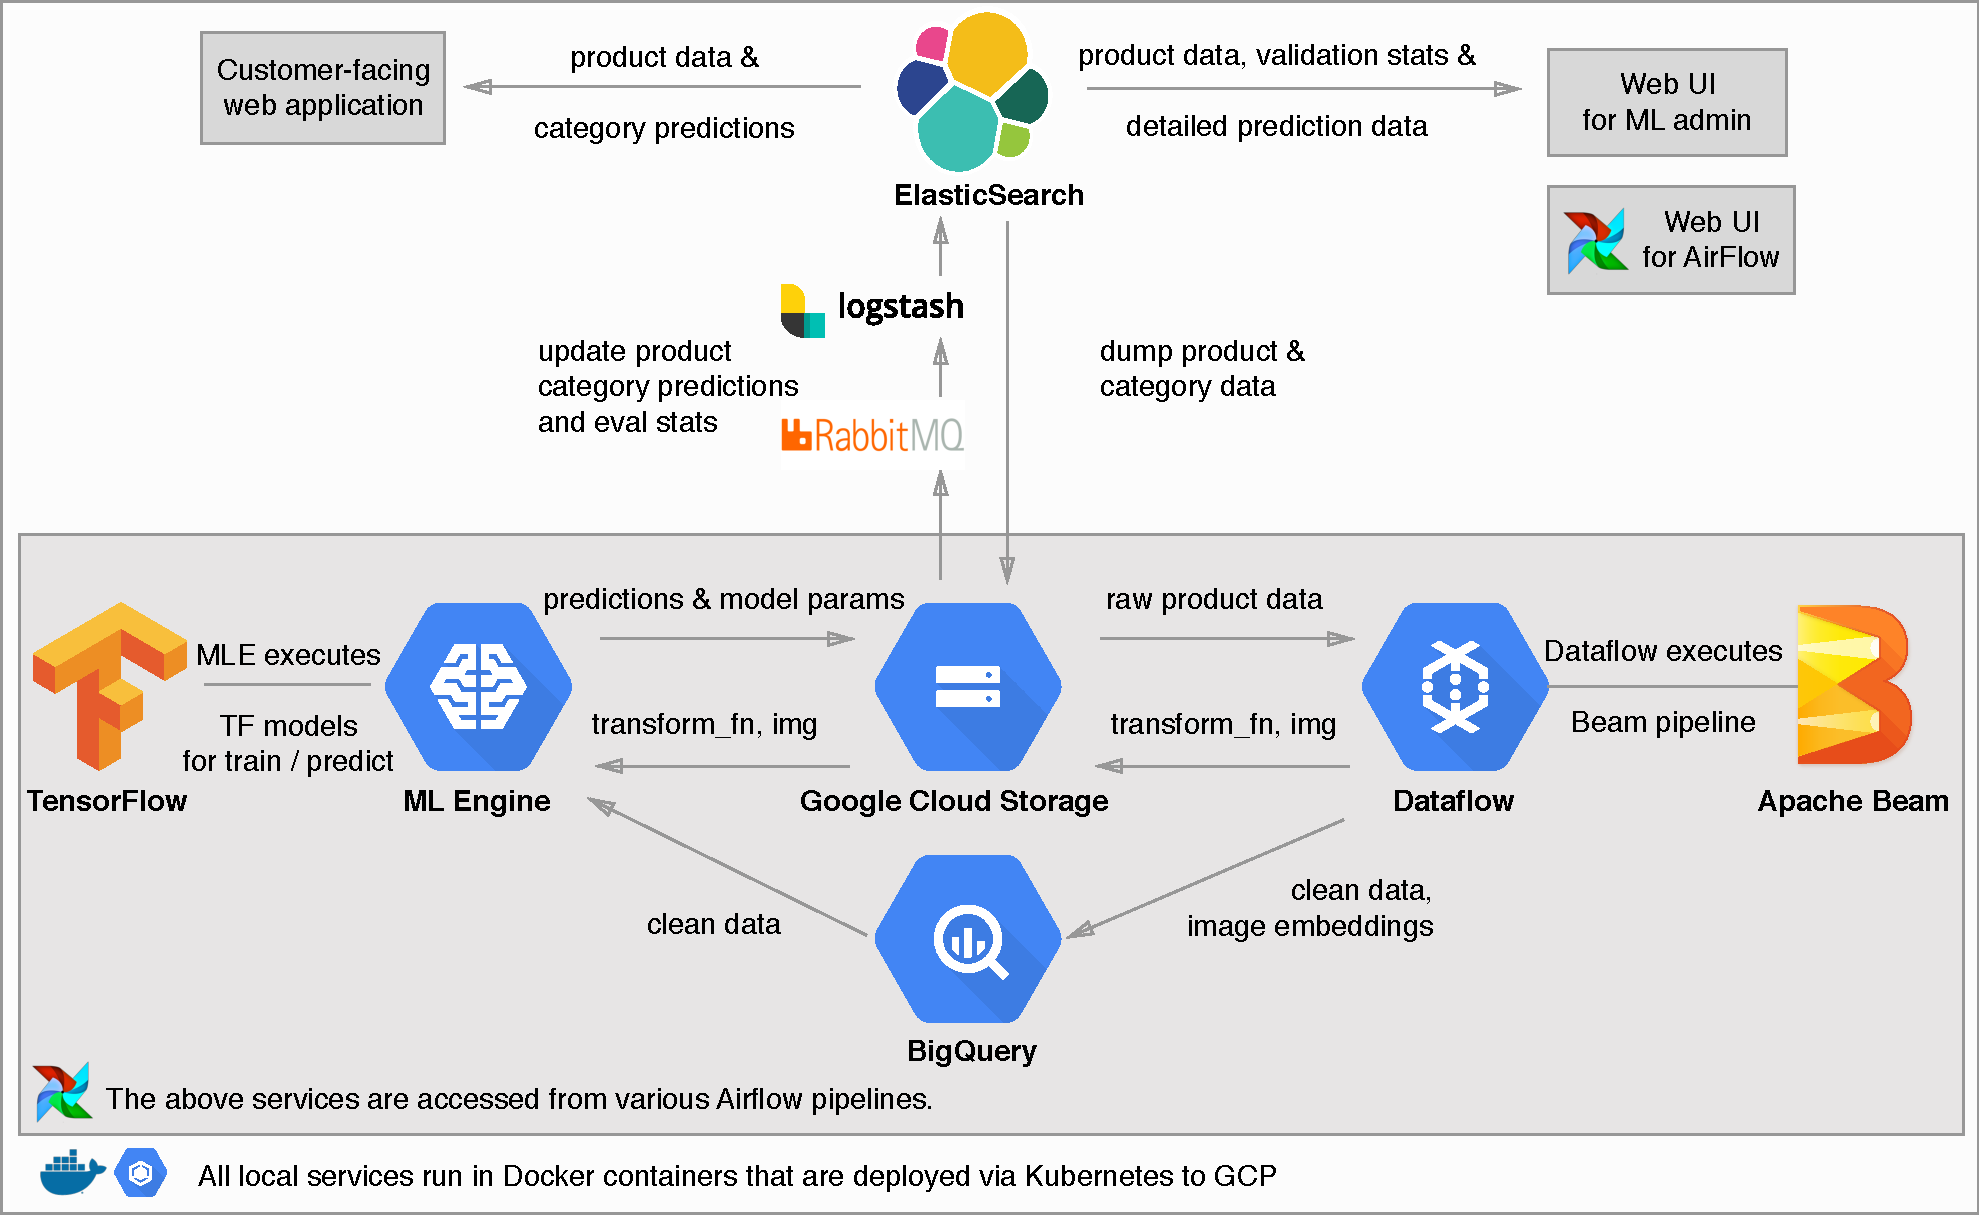
\includegraphics[width=1.4\textwidth]{diagrams/architecture}
  \caption{High-level system architecture of the ML pipeline}
  \label{arch_diagram}
\end{figure}

\section{Experiments}
\subsection{Independent Models}
\label{exp_models}

\subsection{Ensembling}
\label{exp_ensembling}

\subsection{Active Learning}
\label{exp_al}

\subsection{Visual Similarity}
\label{exp_models}


\section{Evaluation}
\label{evaluation}

At the beginning of running all these experiments, the dataset was divided into development and test set (90/10\%).
The development set was used for


 we can evaluate the performance of the model on three types of datasets:

\begin{itemize}
  \item the test or validation set as labelled by the rule-based system (referred to as ``rule-based test/validation set''),
  \item the ground truth dataset gathered  before running most experiments,
  \item
\end{itemize}
